\documentclass[aspectratio=169,11pt]{beamer}

\usepackage[T1]{fontenc}
\usepackage[utf8]{inputenc}
\usepackage{lmodern}
\usepackage{amsmath,amssymb}
\usepackage{booktabs}
\usepackage{array}
\usepackage{tikz}
\usepackage{pgfplots}
\pgfplotsset{compat=1.18}
\usetikzlibrary{arrows.meta,calc,decorations.pathmorphing}

% ---------- black and white style ----------
\usetheme{default}
\setbeamercolor{normal text}{fg=black,bg=white}
\setbeamercolor{structure}{fg=black}
\setbeamercolor{frametitle}{fg=black,bg=white}
\setbeamercolor{title}{fg=black}
\setbeamercolor{subtitle}{fg=black!70}
\setbeamercolor{alerted text}{fg=black}
\setbeamerfont{alerted text}{series=\bfseries}
\setbeamercolor{block title}{fg=white,bg=black}
\setbeamercolor{block body}{fg=black,bg=black!6}
\setbeamerfont{frametitle}{size=\Large,series=\bfseries}
\setbeamertemplate{navigation symbols}{}
\setbeamertemplate{itemize items}[circle]
\setbeamertemplate{blocks}[rounded][shadow=false]
\setbeamertemplate{frametitle}{\vspace{0.35cm}\insertframetitle\par\vspace{-0.1cm}}
\setbeamertemplate{footline}{%
  \hspace{0.5cm}\textcolor{black!55}{\scriptsize CUBICS 2026 \textperiodcentered{} Tethered 6U \textperiodcentered{} Team meeting}%
  \hfill\textcolor{black!55}{\scriptsize\insertframenumber}\hspace{0.5cm}\vspace{0.25cm}}
\setlength{\abovedisplayskip}{4pt}
\setlength{\belowdisplayskip}{4pt}

\newcommand{\meq}{m_{\mathrm{eq}}}

\title{Tethered 6U CubeSat}
\subtitle{What has flown before, how long the tether can be, and 3D photos}
\date{CUBICS 2026 \textperiodcentered{} Stream 1 \textperiodcentered{} Team meeting, October 2026}
\author{}

\begin{document}
\begin{frame}[plain]
  \vfill
  {\Huge\bfseries Tethered 6U CubeSat\par}
  \vspace{0.3cm}
  {\Large What has flown before, how long the tether can be, and 3D photos\par}
  \vspace{0.6cm}
  {\normalsize\color{black!65} CUBICS 2026 \textperiodcentered{} Stream 1 \textperiodcentered{} Team meeting, October 2026\par}
  \vspace{0.4cm}
  {\small\color{black!65} One tether, two 3U halves of 4\,kg, orbit at 550\,km.\par}
  \vfill
\end{frame}
% =====================================================================
\section{Previous work}
% =====================================================================
\begin{frame}{What has flown before}
\centering
\renewcommand{\arraystretch}{1.18}
\begin{tabular}{@{}llll@{}}
\toprule
Mission & Year & Length & What happened \\
\midrule
Gemini XI & 1966 & 30\,m & First tether between two spacecraft \\
SEDS-1 & 1993 & 20\,km & Fully unrolled; the end mass fell back to Earth \\
SEDS-2 & 1994 & 19.7\,km & The tether brake worked as designed \\
TSS-1R & 1996 & 19.7\,km & \textbf{Tether broke (electrical spark)} \\
TiPS & 1996 & 4\,km & Swing reduced from $40^\circ$ to $7.5^\circ$ \\
ATEx & 1999 & 22\,m of 6.2\,km & \textbf{Tether went loose; unrolling stopped} \\
YES2 & 2007 & 31.7\,km & Longest object ever unrolled in orbit \\
TEPCE & 2019 & 1\,km & Two CubeSat halves pushed apart by a spring at 4\,m/s \\
\bottomrule
\end{tabular}

\vspace{0.3cm}
Tethers have flown for 60 years. When they fail, it is almost always while unrolling.
\end{frame}
% =====================================================================
\begin{frame}{Previous tethered systems}
\centering
\begin{tabular}{@{}cc@{}}
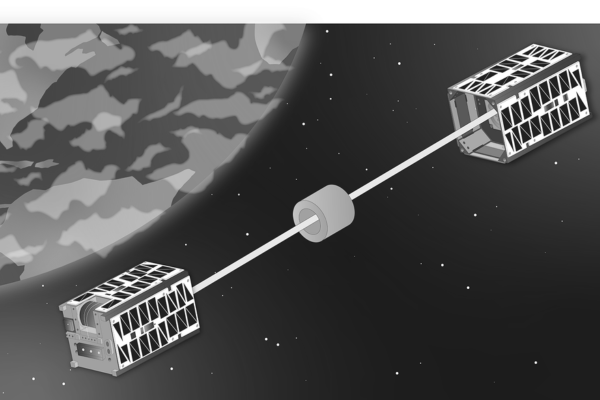
\includegraphics[height=2.75cm]{figs/prior1.png} &
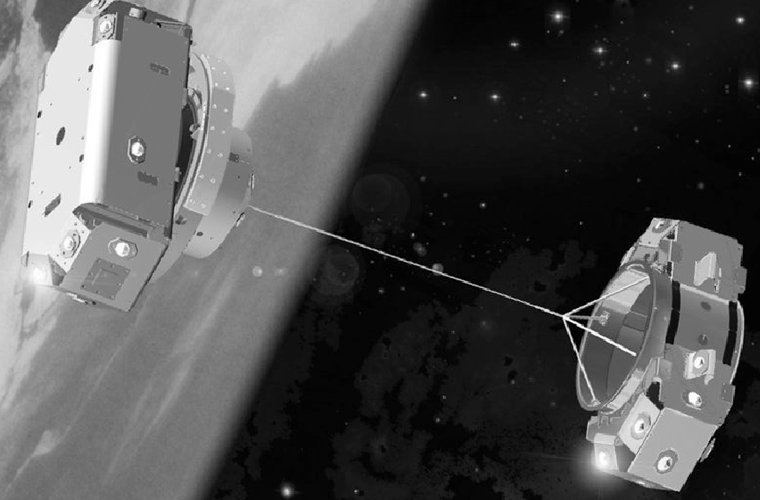
\includegraphics[height=2.75cm]{figs/prior2.png} \\[-2pt]
\footnotesize Two CubeSats joined by a tether &
\footnotesize Two end bodies joined by a tether \\[6pt]
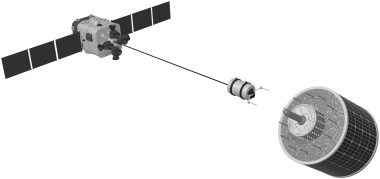
\includegraphics[height=2.2cm]{figs/prior3.png} &
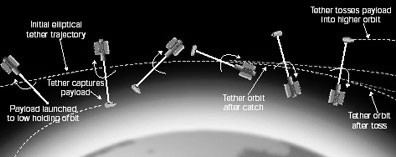
\includegraphics[height=2.2cm]{figs/prior4.png} \\[-2pt]
\footnotesize Tether between a spacecraft and a target &
\footnotesize Momentum exchange: catch and toss \\
\end{tabular}
\end{frame}
% =====================================================================
\begin{frame}{What is already proven, and what is new}
\begin{columns}[T]
\begin{column}{0.47\textwidth}
\begin{block}{Already proven}
\begin{itemize}
\item Splitting a CubeSat in two with a spring (TEPCE, 2019)
\item Unrolling kilometres of tether with a brake (SEDS-2, TiPS)
\item Keeping the pair pointed up and down by gravity alone
\item Calming the swing with the winch
\end{itemize}
\end{block}
\end{column}
\begin{column}{0.47\textwidth}
\begin{block}{New in this proposal}
\begin{itemize}
\item One tether with a winch that unrolls and reels in
\item The tether angle measured at its anchor
\item Tether reeled in between campaigns to last longer
\item Earth photos from both halves
\end{itemize}
\end{block}
\end{column}
\end{columns}
\end{frame}
% =====================================================================
\section{The tether}
% =====================================================================
\begin{frame}{Why the tether stays tight}
\begin{columns}[T]
\begin{column}{0.56\textwidth}
\small
Orbit speed at radius $a = R_\oplus + h$:
\begin{equation*}
n = \sqrt{\frac{\mu}{a^{3}}} = 1.0948\times10^{-3}\ \mathrm{rad/s},\qquad P = \frac{2\pi}{n} = 95.6\ \mathrm{min}.
\end{equation*}
Gravity pulls the lower half a bit more, and the upper half a bit less, than its orbit needs. At a distance $l$ from the centre the difference is
\begin{equation*}
n^{2}(a+l) - \frac{\mu}{(a+l)^{2}} \simeq 3\,n^{2}\,l .
\end{equation*}
The tether makes up the difference, so it pulls with
\begin{equation*}
T = 3\,n^{2}\,\meq\,L,\qquad \meq = \frac{m_1 m_2}{m_1+m_2} = 2\ \mathrm{kg}.
\end{equation*}
\vspace{0.1cm}
\textbf{$T = 3.6$\,mN (500\,m) \quad $T = 7.2$\,mN (1\,km)}
\end{column}
\begin{column}{0.4\textwidth}
\centering
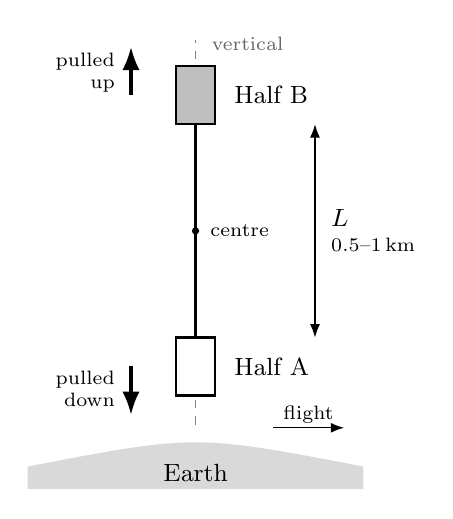
\begin{tikzpicture}[scale=0.82,>=Latex]
  \fill[black!15] (-2.6,-3.55) .. controls (0,-3.05) .. (2.6,-3.55) -- (2.6,-3.9) -- (-2.6,-3.9) -- cycle;
  \node at (0,-3.65) {\small Earth};
  \draw[dashed,black!50] (0,-2.9) -- (0,3.05);
  \node[black!60,font=\scriptsize,anchor=west] at (0.1,3.0) {vertical};
  \draw[thick,fill=black!25] (-0.3,1.75) rectangle (0.3,2.65);
  \draw[thick,fill=white] (-0.3,-2.45) rectangle (0.3,-1.55);
  \draw[thick] (0,1.75) -- (0,-1.55);
  \fill (0,0.1) circle (1.6pt);
  \node[font=\scriptsize,anchor=west] at (0.08,0.1) {centre};
  \node[font=\small,anchor=west] at (0.45,2.2) {Half B};
  \node[font=\small,anchor=west] at (0.45,-2.0) {Half A};
  \draw[->,very thick] (-1.0,2.2) -- (-1.0,2.95);
  \draw[->,very thick] (-1.0,-2.0) -- (-1.0,-2.75);
  \node[font=\scriptsize,align=right,anchor=east] at (-1.1,2.55) {pulled\\ up};
  \node[font=\scriptsize,align=right,anchor=east] at (-1.1,-2.35) {pulled\\ down};
  \draw[<->] (1.85,1.75) -- (1.85,-1.55);
  \node[font=\small,anchor=west,align=left] at (1.95,0.1) {$L$\\[-2pt]\scriptsize 0.5--1\,km};
  \draw[->] (1.2,-2.95) -- (2.3,-2.95);
  \node[font=\scriptsize] at (1.75,-2.75) {flight};
\end{tikzpicture}
\end{column}
\end{columns}
\end{frame}
% =====================================================================
\begin{frame}{It only works up and down}
\small
Motion of one half seen from the other ($x$ up, $y$ forward, $z$ sideways):
\begin{equation*}
\ddot{x} - 2n\dot{y} - 3n^{2}x = f_x,\qquad
\ddot{y} + 2n\dot{x} = f_y,\qquad
\ddot{z} + n^{2}z = f_z .
\end{equation*}
\vspace{-0.2cm}
\begin{center}
\renewcommand{\arraystretch}{1.3}
\begin{tabular}{@{}lll@{}}
\toprule
Direction & What happens & Tether \\
\midrule
Up and down ($x$) & $+3n^{2}x$: the halves pull apart & tight \\
Forward and back ($y$) & no force at all & loose \\
Sideways ($z$) & $-n^{2}z$: the halves drift together & loose \\
\bottomrule
\end{tabular}
\end{center}
A tilted tether swings back to vertical:
\begin{equation*}
\ddot{\varphi} + 3n^{2}\sin\varphi\cos\varphi = 0
\;\Rightarrow\;
\text{swing period } \frac{2\pi}{\sqrt{3}\,n} = 55\ \mathrm{min}.
\end{equation*}
\alert{A diagonal tether is a swing, not a position.} Holding $30^\circ$ at 1\,km needs
$3n^{2}\meq L^{2}\sin\varphi\cos\varphi = 3.1$\,N\,m, about 3000 times what a CubeSat wheel gives.
\end{frame}
% =====================================================================
\begin{frame}{500 m or 1 km with one tether: the numbers}
\centering
\renewcommand{\arraystretch}{1.25}
\begin{tabular}{@{}lccc@{}}
\toprule
 & Formula & $L = 500$\,m & $L = 1$\,km \\
\midrule
Pull on the tether & $3n^{2}\meq L$ & 3.6\,mN & 7.2\,mN \\
Stretch & $TL/(EA)$ & 0.6\,mm & 2.3\,mm \\
Tether mass, 0.2\,mm thick & $\rho_c A L$ & 22\,g & 44\,g \\
Area facing the air flow & $d\,L$ & 0.10\,m$^{2}$ & 0.20\,m$^{2}$ \\
Time to unroll, slowly & $\ln(L/L_0)/\lambda$ & 3.2\,h & 3.5\,h \\
Time to reel in, slowly & $\ln(L/L_0)/\lambda$ & 7.9\,h & 8.8\,h \\
Time in orbit, tether out & drag model & $\approx 2.5$\,years & $\approx 1.6$\,years \\
\bottomrule
\end{tabular}

\vspace{0.25cm}
{\footnotesize\color{black!65} $EA = 3142$\,N, $L_0 = 1$\,m, $\lambda = n/2$ out and $n/5$ in, average Sun. Tether reeled in: $\approx 6$\,years.}
\end{frame}
% =====================================================================
\begin{frame}{Once out, the length stays fixed}
The winch sets the length. More pull does not make the tether longer; it only makes it tighter.
\vspace{0.3cm}
\begin{columns}[T]
\begin{column}{0.4\textwidth}
\begin{block}{Stretch}
\centering
$\Delta L = \dfrac{T\,L}{EA}$\\[4pt]
{\Large\bfseries $\le$ 2.3\,mm}\\[2pt]
\footnotesize at 1\,km
\end{block}
\end{column}
\begin{column}{0.4\textwidth}
\begin{block}{Natural swing}
\centering
$2\pi/(\sqrt{3}\,n)$\\[4pt]
{\Large\bfseries 55\,min}\\[2pt]
\footnotesize one slow swing around vertical
\end{block}
\end{column}
\end{columns}
\vspace{0.4cm}
The pull depends only on the length: $T = 3n^{2}\meq L$. Unrolling faster only adds swing and more braking.
\end{frame}
% =====================================================================
\begin{frame}{Angle between the halves: use the mechanism}
\begin{columns}[c]
\begin{column}{0.56\textwidth}
\begin{itemize}
\setlength{\itemsep}{8pt}
\item The tether already points from one half to the other.
\item A free joint at each anchor, with angle sensors, reads that direction.
\item It is a mechanical measurement: it does not drift and needs no extra electronics.
\item When the two halves are joined, the angle is zero: that is our calibration.
\end{itemize}
\end{column}
\begin{column}{0.4\textwidth}
\centering
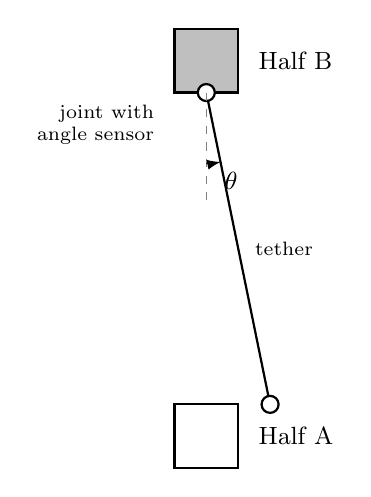
\begin{tikzpicture}[scale=0.9,>=Latex]
  \draw[thick,fill=black!25] (-0.45,2.2) rectangle (0.45,3.1);
  \draw[thick,fill=white] (-0.45,-3.1) rectangle (0.45,-2.2);
  \draw[thick] (0,2.2) -- (0.9,-2.2);
  \draw[thick,fill=white] (0,2.2) circle (0.12);
  \draw[thick,fill=white] (0.9,-2.2) circle (0.12);
  \draw[dashed,black!50] (0,2.2) -- (0,0.6);
  \draw[->] (0,1.2) arc (-90:-78.4:1.0);
  \node[font=\small] at (0.35,0.95) {$\theta$};
  \node[font=\small,anchor=west] at (0.6,2.65) {Half B};
  \node[font=\small,anchor=west] at (0.6,-2.65) {Half A};
  \node[font=\scriptsize,anchor=east,align=right] at (-0.6,1.75) {joint with\\ angle sensor};
  \node[font=\scriptsize,anchor=west] at (0.55,0.0) {tether};
\end{tikzpicture}
\end{column}
\end{columns}
\end{frame}
% =====================================================================
\section{3D photos}
% =====================================================================
\begin{frame}{3D photos need two very different viewing angles}
\begin{columns}[c]
\begin{column}{0.55\textwidth}
\centering
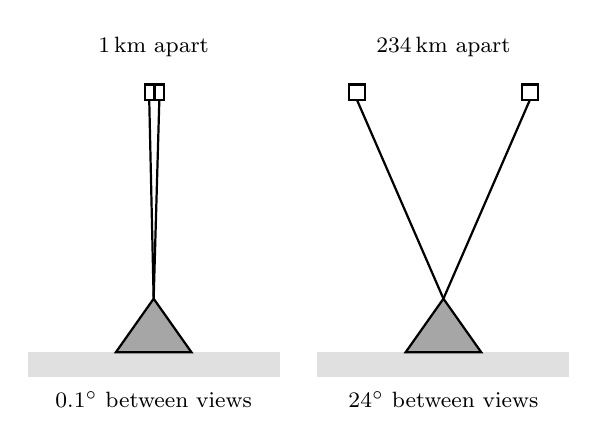
\begin{tikzpicture}[scale=0.8,>=Latex]
  % left: tether baseline
  \begin{scope}
    \fill[black!12] (-2,-0.4) rectangle (2,0);
    \draw[thick,fill=black!35] (-0.6,0) -- (0,0.85) -- (0.6,0) -- cycle;
    \draw[thick,fill=white] (-0.14,4.0) rectangle (0.0,4.25);
    \draw[thick,fill=white] (0.02,4.0) rectangle (0.16,4.25);
    \draw[thick] (-0.07,4.0) -- (0,0.85);
    \draw[thick] (0.09,4.0) -- (0,0.85);
    \node[font=\footnotesize,align=center] at (0,4.85) {1\,km apart};
    \node[font=\footnotesize] at (0,-0.75) {$0.1^\circ$ between views};
  \end{scope}
  % right: fore/aft
  \begin{scope}[xshift=4.6cm]
    \fill[black!12] (-2,-0.4) rectangle (2,0);
    \draw[thick,fill=black!35] (-0.6,0) -- (0,0.85) -- (0.6,0) -- cycle;
    \draw[thick,fill=white] (-1.5,4.0) rectangle (-1.25,4.25);
    \draw[thick,fill=white] (1.25,4.0) rectangle (1.5,4.25);
    \draw[thick] (-1.37,4.0) -- (0,0.85);
    \draw[thick] (1.37,4.0) -- (0,0.85);
    \node[font=\footnotesize,align=center] at (0,4.85) {234\,km apart};
    \node[font=\footnotesize] at (0,-0.75) {$24^\circ$ between views};
  \end{scope}
\end{tikzpicture}
\end{column}
\begin{column}{0.42\textwidth}
A point of height $h$ shifts between the photos by
\begin{equation*}
p = h\,\frac{B}{H},
\end{equation*}
so the height error is
\begin{equation*}
\sigma_h = \frac{\sigma_p}{B/H}.
\end{equation*}
$B$: distance between the two photos, $H = 550$\,km, $\sigma_p$: how well the photos can be matched (1.5\,m with 5\,m pixels).
\end{column}
\end{columns}
\end{frame}
% =====================================================================
\begin{frame}{With the tether, the height error is about 1 km}
Even if the tether were horizontal, the photos are only $L$ apart: $B/H = L/H$ (5\,m pixels).
\vspace{0.4cm}
\begin{columns}[T]
\begin{column}{0.31\textwidth}
\begin{block}{$L = 1$\,km}
\centering
{\Large\bfseries $\sigma_h \approx 825$\,m}\\[2pt]
\footnotesize height error
\end{block}
\end{column}
\begin{column}{0.31\textwidth}
\begin{block}{$L = 500$\,m}
\centering
{\Large\bfseries $\sigma_h \approx 1.65$\,km}\\[2pt]
\footnotesize height error
\end{block}
\end{column}
\begin{column}{0.31\textwidth}
\begin{block}{1\,km-high mountain}
\centering
{\Large\bfseries 0.36 pixel}\\[2pt]
\footnotesize shift between the two photos
\end{block}
\end{column}
\end{columns}
\vspace{0.5cm}
With a vertical tether it is worse: both cameras look along the same line, so there is no 3D at all.
\end{frame}
% =====================================================================
\begin{frame}{What works: pointing the cameras}
\centering
\renewcommand{\arraystretch}{1.35}
\small
\begin{tabular}{@{}lccl@{}}
\toprule
Option & $B/H$ & Height error & Where \\
 & & (5\,m / 20\,m pixels) & \\
\midrule
A $12^\circ$ ahead, B $12^\circ$ back & 0.43 & 3.5\,m / 14\,m & Under the track \\
Turning camera, $\pm30^\circ$ & 0.40 & 3.8\,m / 15\,m & Any site, every 2--4 days \\
Tether, 1\,km apart & $1.8\times10^{-3}$ & 825\,m / 3.3\,km & \textbf{Not usable} \\
\bottomrule
\end{tabular}

\vspace{0.5cm}
\begin{block}{}
\centering The 3D comes from the satellite moving 234\,km along its orbit in 31\,s, not from the tether.
\end{block}
\end{frame}
% =====================================================================
\section{Wrap-up}
% =====================================================================
\begin{frame}{Risks}
\renewcommand{\arraystretch}{1.45}
\begin{tabular}{@{}>{\bfseries\raggedright\arraybackslash}p{3.0cm}p{10.4cm}@{}}
\toprule
Reeling in & Reeling in makes the swing grow. It must be slow and controlled: 7.9 to 8.8\,h. \\
Time in orbit & Reel the tether in when not in use: about 6 years instead of 1.6 at 550\,km. Let it out at the end to fall back faster. \\
One tether & One cut by a tiny piece of debris ends the mission. Use a braided line. \\
Space rules & A 1\,km object is a bigger target for collisions. Check with the CSA that it is accepted. \\
Our estimates & Orbit times come from a simple model; a proper study (STELA or DRAMA) is needed. \\
\bottomrule
\end{tabular}
\end{frame}
% =====================================================================
\begin{frame}{In short}
\renewcommand{\arraystretch}{1.5}
\begin{tabular}{@{}>{\bfseries\raggedright\arraybackslash}p{3.0cm}p{10.4cm}@{}}
\toprule
Previous work & Tethers have flown since 1966. Most failures happen while unrolling. \\
Tether length & Only up and down. 500\,m to 1\,km works: 3.6 to 7.2\,mN of pull, about 3.5\,h to unroll. \\
Angle between halves & Measured by the mechanism at the anchor, not by electronics that drift. \\
3D photos & Not with the tether: errors near 1\,km. Yes by pointing the cameras: about 3.5\,m. \\
Time in orbit & Reel the tether in when not in use: about 6 years instead of 1.6. \\
\bottomrule
\end{tabular}
\end{frame}
% =====================================================================
\begin{frame}{Decisions for the team}
\renewcommand{\arraystretch}{1.6}
\begin{tabular}{@{}>{\bfseries}l p{12.3cm}@{}}
1 & \textbf{Tether length}: 500\,m or 1\,km, reeled in between campaigns. \\
2 & \textbf{Angle between halves}: joint with angle sensors at each anchor. \\
3 & \textbf{3D photos}: drop 3D from the tether; point the cameras instead. \\
4 & \textbf{Questions to the CSA by 9 November}: launch height, is the tether accepted, how it falls back. \\
5 & \textbf{Study}: proper orbit-time study with STELA or DRAMA. \\
\end{tabular}
\end{frame}

\end{document}
